\section{Differentialgleichungssysteme}

\subsection{Matrixdarstellung}
Für ein $n$-dimensionales DGL-System 1. Ordnung
\begin{equation*}
    \left.
    \begin{array}{ll}
        x_1'(t) &= f_1(t,x_1(t),\ldots,x_n(t)) \\
        &\hspace{1mm}\vdots \\
        x_n'(t) &= f_n(t,x_1(t),\ldots,x_n(t)) \\
    \end{array}
    \right\}
    x'(t) = f(t,x(t))
    \qquad \text{mit AB} \quad
    \left.
    \begin{array}{ll}
        x_1(t_0) &= x_{1,0} \\
        &\hspace{1mm}\vdots \\
        x_n(t_0) &= x_{n,0} \\
    \end{array}
    \right\}
    x(t_0) = x_0    
\end{equation*}
kann falls \emph{$f$ linear} eine Matrixform aufgestellt werden:
\[ x' = Ax + b \]

Das System is autonom, falls alle $a_{ij}$ konstant und homogen falls alle $b_i=0$.

Kritische Punkte: $x' = Ax + b = 0$, Gleichgewicht: $b = -Ax$ oder $x = -A^{-1}*b$\\
Lösungen bei b=0 (homogenen Gleichung): Für jeden Eigenwert und Eigenvektor eine Lösung: \\
\begin{enumerate}[label=\alph*)]
    \item Ist $\lambda$ ein einfacher reeller Eigenwert von $A$ mit Eigenvektor $\textbf{v}$, so ist die Lösung: $x(t) = C \cdot e^{\lambda t}\textbf{v}$ 
    \item Ist $\lambda$ ein $k$-facher reeler Eigenwert von $A$, so ist die Lösung: \\ \begin{equation*}
    	\textbf{x}_1(t) = C_1 \cdot e^{\lambda t}\textbf{p}_0(t), \quad \textbf{x}_2(t) = C_2 \cdot e^{\lambda t}\textbf{p}_1(t), \quad \dots, \quad \textbf{x}_k(t) = C_k \cdot e^{\lambda t} \textbf{p}_{k-1}(t)
    \end{equation*}
    Falls es nur einen einzigen (linear unabhängigen) Eigenvektor $\textbf{v}$ gibt, muss noch ein \textit{verallgemeinerter Eigenvektor} gefunden werden (wenn 2. Ordnung).
    \begin{equation*}
    	(A - \lambda E_n)\textbf{p}^* = \textbf{v} \Rightarrow (A-\lambda E_n)^2 \textbf{p}^* = 0
    \end{equation*}
    \item Ist $\lambda = \mu + j\nu$ ein einfacher echt komplexer Eigenwert ($\nu \neq 0$) von $A$ und $\textbf{v} = a + jb$ ein Eigenvektor von $A$, so ist die Lösung: \\
    \begin{equation*}
		x(t) = e^{\lambda t}\textbf{v} = e^{(\mu + j\nu)t} \left(a + jb\right)
    \end{equation*}
    \begin{equation*}
    	\textbf{z}_1(t) = \operatorname{Re} (e^{\lambda t \textbf{v}}) = C_1 \cdot e^{\mu t} \left(a \cos(\nu t) - b \sin(\nu t)\right)
    \end{equation*}
	\begin{equation*}
    	\textbf{z}_2(t)= \operatorname{Im} (e^{\lambda t \textbf{v}}) = C_2 \cdot e^{\mu t} \left(a \sin(\nu t) + b \cos(\nu t)\right)
    \end{equation*}
    \item Ist $\lambda = \mu + j\nu$ ein mehrfacher echt komplexer eigenwert von $A$, so müssen Fall b) und c) kombiniert werden.
\end{enumerate}

\subsection{Variation der Konstanten}
Gegeben ist ein lineares, inhomogenes System 1. Ordnung: \\
\begin{equation*}
\frac{d}{dt}x(t) = Ax(t) + b(t) 
\end{equation*}
Als erstes werden die Lösungen der homogenen Gleichung gelöst, wir erhalten für jeden Eigenwert und Eigenvektor eine Lösung: 
$x_1(t) = e^{\lambda_1t}v_1,x_2(t) = e^{\lambda_2t}v_2...x_n(t) = e^{\lambda_nt}v_n$. 
Diese Lösungen ergeben unsere \emph{Fundamentalmatrix}:\\
\begin{equation*}
X(t) = 
	\begin{bmatrix} 
	        x_1(t) && x_2(t) && ... && x_n(t)\\    
	\end{bmatrix}
\end{equation*}

Mit Hilfe der Fundamentalmatrix können wir nun die partikuläre Lösung des Systems bestimmen:\\
\begin{equation*}
y_P(t) = X(t) \int{X(t)^{-1}b(t)dt}
\end{equation*}
Die gesamte Lösung ist nun die Summe der homogenen und der partikulären Lösung $y(t) = y_h(t) + y_p(t)$.


\subsection{Superpositionsprinzip}
Gegeben ist folgendes lineares homogenes Gleichungssystem:
\begin{equation*}
\frac{d}{dt}x(t) = A(t)x(t)
\end{equation*}
Das Superpositionsprinzip sagt, dass die Linearkombination der beiden Lösungen $x_1(t)$ und $x_2(t)$ auch wieder eine Lösung des Differentialgleichungssystems ist. 
\begin{equation*}
	x(t) = c_1 x_1(t) + c_2 x_2(t)
\end{equation*}
Wobei $c_1$ und $c_2$ beliebige Skalare sind. 
Das Prinzip kann auch für Systeme höherer Ordnung verwendet werden. \\

Hier ein \textbf{Beispiel} für eine Differentialgleichung zweiter Ordnung: \\
Gegeben: $t^2y''(t)-4ty'(t)+6y(t)=0$, $t>0$, $y_1(t)=t^2$\\
Gesucht: Eine zweite Lösung $y_2(t)$, so dass ${y_1(t),y_2(t)}$ ein Fundamentalsystem ergeben. \\
Vorgehensweise: \\
\textbf{Schritt 1:}\\
Prüfen, ob $y_1(t)$ wirklich Lösung des Systems ist. \\
\textbf{Schritt 2:}\\
Für die zu bestimmende Lösung $y_2(t)$ kommt folgender Ansatz zum Zug: $y_2(t) = v(t)y_1(t)$.\\
\textbf{Schritt 3:}\\
Ansatz $v(t)y_1(t)$ in Differentialgleichung einsetzen. Die Gleichung so weit es geht umformen und danach nach $v(t)$ auflösen. Wenn $v(t)$ bekannt ist, kann $y_2(t)$ berechnet werden. \\
\textbf{Schritt 4:}\\
Auf Grund der beiden Lösungen, kann die Fundamentalmatrix $Y(t) =
\begin{vmatrix} 
	        y_{1}(t) & y_{2}(t)\\ 
	        y'_{1}(t) & y'_{2}(t)\\   
\end{vmatrix} $ berechnet werden und mit Hilfe der Wronskideterminante geprüft werden, ob die Lösungen linear unabhängig sind ($det(W) \neq 0$). 

\subsection{Lineare Unabhängigkeit}
Die lineare Unabhängigkeit der beiden Lösungen $x_1(t)$ und $x_2(t)$ kann mit Hilfe der \textbf{Wronskideterminante} geprüft werden. 
\begin{equation*}
	W(t) = det[X(t)] =    
	\begin{vmatrix} 
	        x_{11}(t) & x_{12}(t)\\ 
	        x_{21}(t) & x_{22}(t)\\   
	\end{vmatrix}
\end{equation*}
Sind $x_1(t)$ und $x_2(t)$ \textbf{linear unabhängig}, dann gilt $W(t) \neq 0$ für alle $t \in I$. \\
Sind $x_1(t)$ und $x_2(t)$ \textbf{linear abhängig}, dann gilt $W(t) = 0$ für alle $t \in I$. \\
Jede Lösung $\Phi(t)$ kann als Linearkombination eines Fundamentalsystems zweier Lösungen $x_1(t)$ und $x_2(t)$ dargestellt werden. Diese Linearkombination wird als die allgemeine Lösung eines linearen homogenen Systems bezeichnet. \\
\textbf{Theorem von Abel}\\
\begin{equation*}
W(t) = c\cdot e^{\int{\operatorname{trace}(A(t))dt}}
\end{equation*}
Spur einer Matrix = Summe der Hauptdiagonalelemente

\subsection{Fluss eines Vektorfeldes / Matrixexponential}
Für ein AWP $x'(t) = A(t) x(t)$ mit $x(t_0)=x_0$ wird der Fluss $\Phi(t)$ so definiert, dass 
\[ x(t) = \Phi(t) \cdot x_0 \]
Dafür müssen $\Phi'(t) = A(t)\Phi(t)$ und $\Phi(t_0) = E$ erfüllt sein.
Daraus folgt das \emph{Matrixexponential} von $A$:

\[
    \Phi(t) = X(t)X(t_0)^{-1} = e^{At} = \sum\limits_{k=0}^{\infty}\frac{(At)^k}{k!}
\]

Damit hat die Lösung x(t) des Anfangswertproblems $x(0) = x_0$ folgende Form: 
\[
    x(t) = e^{At}x_0
\]


Beispiele:\\
Gegeben: $A = 	\begin{vmatrix} 
	        		\lambda & 0\\ 
	        		0 & \lambda\\   
				\end{vmatrix} 
				\rightarrow$ 
$e^{tA} = \begin{vmatrix} 
	        		e^{t\lambda} & 0\\ 
	        		0 & e^{t\lambda}\\   
				\end{vmatrix}$\\
Gegeben: $A = 	\begin{vmatrix} 
	        		\lambda & 1\\ 
	        		0 & \lambda\\   
				\end{vmatrix} 
				\rightarrow$ 
$e^{tA} = \begin{vmatrix} 
	        		e^{t\lambda} & te^{t\lambda}\\ 
	        		0 & e^{t\lambda}\\   
				\end{vmatrix}$\\
				
Gegeben: $A = 	\begin{vmatrix} 
	        		2 & 3\\ 
	        		3 & 2\\   
				\end{vmatrix} \rightarrow
				\lambda_1=5 \; \lambda_2=-1 \rightarrow ev_1=\begin{vmatrix}
					1\\ 
					1\\   
				\end{vmatrix} \;
				ev_2=\begin{vmatrix}
					1\\ 
					-1\\   
				\end{vmatrix} \rightarrow
				T=\begin{vmatrix} 
	        		1 & 1\\ 
	        		1 & -1\\   
				\end{vmatrix} \rightarrow 
				B=T^{-1} \cdot A \cdot T=\begin{vmatrix} 
	        		5 & 0\\ 
	        		0 & -1\\   
				\end{vmatrix} \rightarrow$\\
				\hspace*{4cm}$e^{tA}=T \cdot e^{tB} \cdot T^{-1}=
				T \cdot \begin{vmatrix} 
					e^{5 t} & 0\\ 
					0 & e^{-t}\\   
				\end{vmatrix} \cdot T^{-1} =
				\dfrac{1}{2}\begin{vmatrix} 
					e^{5 t} + e^{-t}& e^{5 t} - e^{-t}\\ 
					e^{5 t} - e^{-t} & e^{5 t} + e^{-t}\\   
				\end{vmatrix}$

\subsection{Degenerierte Matrizen}
Ist $A$ degeneriert, bedeutet dies, dass sie mindestens einen Eigenwert $\lambda$ mit einer geometrischen Vielfachheit (Anzahl Eigenvektoren) besitzt, die kleiner als seine algebraische Vielfachheit (Anzahl gleiche Eigenwerte $m$) ist. 
Das bedeutet, dass die linear unabhängigen Eigenvektoren der Matrix $A$ den Raum $\mathbb{R}^n$ nicht ausschöpft.\\
Ist $\lambda$ ein Eigenwert von $A$ mit der algebraischen Vielfachheit $m$, dann besitzt die Gleichung: 
\begin{equation*}
(A-\lambda E)^m b_k = 0
\end{equation*}
eine Anzahl $m$ linear unabhängige Lösungen $b_1$ bis $b_m$ und für $k = 1,\ldots,m$ sind die vektorwertigen Funktionen
\begin{equation*}
x_k(t) = e^{\lambda t}\left[{b_k + \frac{t}{1!}(A-\lambda E)b_k + ... + \frac{t^{m-1}}{(m-1)!}(A-\lambda E)^{m-1}b_k}\right]
\end{equation*}
\begin{equation*}
 \Longrightarrow x_k(t) = e^{\lambda t}(b_k + t (A-\lambda E) b_k))
\end{equation*}
linear unabhängige Lösungen der Differentialgleichung. 
\subsection{Beispiel}
Folgende Matrix A ist gegeben: 
\begin{equation*}
	A =     
\begin{bmatrix} %phantom is for spacing
	2 & 0 & -1\\
	0 & 3 & 1\\
	0 & 0 & 2\\
\end{bmatrix}
\end{equation*}
\begin{equation*}
\det(A-\lambda E) = 0 \qquad \Longrightarrow \lambda_1 = 2 \text{(Doppelt)} \quad \lambda_2 = -1
\end{equation*}

\textbf{Schritt 1:} Eigenvektoren berechenen (Hier im Beispiel nur für $\lambda_1$)\\
\begin{equation*}
(A - \lambda_1 E)\nu = 0 \qquad \Longrightarrow \nu = 
\begin{bmatrix} %phantom is for spacing
	1 \\
	0 \\
	0 \\
\end{bmatrix}
\end{equation*}


\begin{equation*}
\Longrightarrow \text{Nur ein Eigenvektor aber zwei Eigenwerte $\lambda_1 = 2$} \quad \Longrightarrow m = 2
\end{equation*}
\textbf{Schritt 2:} Basisvektorern $b_k$ bestimmen \\
\begin{equation*}
(A-\lambda E)^2 b_k = 0 \qquad \Longrightarrow 0\cdot b_{k1} + 9\cdot b_{k2} - 3\cdot b_{k3} = 0
\end{equation*}
\begin{equation*}
b_1= 
\begin{bmatrix} %phantom is for spacing
	1 \\
	0 \\
	0 \\
\end{bmatrix}
\qquad b_2= 
\begin{bmatrix} %phantom is for spacing
	0 \\
	1 \\
	3 \\
\end{bmatrix}
\end{equation*}
\textbf{Schritt 3:} Lösung bestimmen\\
\begin{equation*}
x_1(t) = e^{2 \cdot t} (b_1 + t(A -  2 E)b_1) \qquad \Longrightarrow e^{2\cdot t}
\begin{bmatrix} %phantom is for spacing
	1 \\
	0 \\
	0 \\
\end{bmatrix}
\end{equation*}
\begin{equation*}
x_2(t) = e^{2 \cdot t} (b_2 + t(A -  2  E)b_2) \qquad \Longrightarrow e^{2\cdot t}
\begin{bmatrix} %phantom is for spacing
	-3t \\
	1 \\
	3 \\
\end{bmatrix}
\end{equation*}
\begin{equation*}
 \Longrightarrow X(t) = 
\begin{bmatrix} %phantom is for spacing
	 x_1(t) & x_2(t) \\
\end{bmatrix}
=
\begin{bmatrix} %phantom is for spacing
	1 \cdot e^{2 \cdot t} & -3t \cdot e^{2 \cdot t} \\
	0 & 1\cdot e^{2 \cdot t}  \\
	0 & 3 \cdot e^{2 \cdot t} \\
\end{bmatrix}
\end{equation*}

\subsection{Umwandlung in ein System 1. Ordnung}\label{2to1}
Skalare, lineare, homogene DGL 2. Ordnung mit konstanten Koeffizienten:
\[a \cdot y''(t) + b \cdot y'(t) + c \cdot y(t) = 0 \]
Substitution: \qquad $x_1(t) = y(t) \qquad \text{und} \qquad x_2(t) = y'(t)$\\
\[
	\begin{vmatrix} 
	        y'(t)\\ 
	        y''(t)\\   
	\end{vmatrix}
	=
	\begin{vmatrix} 
	        x_1'(t)\\ 
	        x_2'(t)\\   
	\end{vmatrix}
	=
	\begin{vmatrix} 
	        x_2(t)\\ 
	        -\frac{b}{a} - \frac{c}{a}x_1(t)\\   
	\end{vmatrix}
\]
ergibt das DGL System:\\
\begin{equation*}
x'(t) = Ax(t)
\end{equation*}
\begin{equation*}
	\begin{vmatrix} 
	        x_1'(t)\\ 
	        x_2'(t)\\   
	\end{vmatrix}
	=
	\begin{vmatrix} 
	        0 && 1\\ 
	       -\frac{c}{a} && -\frac{b}{a}\\   
	\end{vmatrix}
	\begin{vmatrix} 
	        x_1(x)\\ 
	        x_2(x)\\   
	\end{vmatrix}
\end{equation*}

Das DGL System kann nun wie ein homogenes, autonomes DGL System 1. Ordnung gelöst werden. Die Lösung für $x_1(t)$ ist geraade die Lösung der DGL 2. Ordnung, weil $x_1(t) = y(t)$, die Lösung $x_2(t)$ kann als Zwischenresultat betrachtet werden. 
Hat das DGL System 2.Ordnung noch eine Störung $g(t)$, so sieht das äquivalente System 1. Ordnung wie folgt aus:\\
\begin{equation*}
x'(t) = Ax(t) + g(t)
\end{equation*}
\begin{equation*}
	\begin{vmatrix} 
	        x_1'(t)\\ 
	        x_2'(t)\\   
	\end{vmatrix}
	=
	\begin{vmatrix} 
	        0 && 1\\ 
	       -\frac{c}{a} && -\frac{b}{a}\\   
	\end{vmatrix}
	\begin{vmatrix} 
	        x_1(t)\\ 
	        x_2(t)\\   
	\end{vmatrix}
	+
	\begin{vmatrix} 
	        0\\ 
	        g(t)\\   
	\end{vmatrix}
\end{equation*}

\paragraph{Transformation 3.Ordnung} $y'''(t) + p(t)y''(t)+q(t)'(t)+r(t)y(t)=g(t)$:\\
\begin{equation*}
	\begin{vmatrix} 
	        x_1(t)\\ 
	        x_2(t)\\
	        x_3(t)   
	\end{vmatrix}
	=
	\begin{vmatrix} 
	        y(t)\\ 
	        y'(t)\\
	        y''(t)   
	\end{vmatrix}
\end{equation*}
\begin{equation*}
	\begin{vmatrix} 
	        x_1'(t)\\ 
	        x_2'(t)\\
	        x_3'(t)   
	\end{vmatrix}
	=
	\begin{vmatrix} 
	        0 && 1 && 0\\ 
	        0 && 0 && 1\\
	        -r(t) && -q(t) && -p(t)   
	\end{vmatrix}
		\begin{vmatrix} 
		        x_1(t)\\ 
		        x_2(t)\\
		        x_3(t)   
		\end{vmatrix}
		+
			\begin{vmatrix} 
			        0)\\ 
			        0\\
			        g(t)   
			\end{vmatrix}
\end{equation*}

\subsection{Zweite Lösung finden für DGL 2. Ordnung}
Gegeben: Diffgleichung 2. Ordnung mit Lösung, suche eine zweite Lösung.\\
Vorgehen:\\
1. Prüfe, ob erste Lösung $y_1(t)=t^2$ für $t^2y''(t) -4ty(t) +6y(t) = 0$ wirklich Lösung ist. \\
2. Ansatz $y_2(t)=v(t)\cdot y_1(t)$ in DGL einsetzen. \\
3. $v''(t),v'(t),v(t)$ ordnen und $v(t)$ berechnen. \\
4. $y_2(t)=v(t)\cdot y_1(t)$ berechnen und prüfen, obs stimmt.\\
5. Fundamentalmatrix $Y(t) = 	\begin{vmatrix} 
	        						y_1(t) && y_2(t)\\ 
	        						y_1'(t) && y_2'(t)\\ 
								\end{vmatrix}$
berechnen und Wronskideterminante prüfen. 


\subsection{Verschiedene Lösungsansätze für inhomogene lineare Systeme }
\subsubsection{Elimination einer Variablen}

Gegenteil von \ref{2to1}. Aus zwei 1. Ordnungen wird eine 2. Ordnung. Nicht sehr elegant, je nachdem aber sehr effektiv. Anschliessend wie für 2. Ordnung rechnen.

\subsubsection{Entkoppeln}
\begin{equation*}
	A = TDT^{-1} 
\end{equation*}
\begin{equation*}
	D = \mathrm{diag}(\lambda_1, \lambda_2, \dots, \lambda_n)
\end{equation*}
\begin{equation*}
	T = (v_1, v_2, \dots, v_n)
\end{equation*}
\begin{equation*}
	\dot{x} = Ax \rightarrow \dot{x} = TDT^{-1}x \Rightarrow T^{-1}\dot{x} = DT^{-1}x \rightarrow y = T^{-1}x \Rightarrow x = Ty
\end{equation*}

\subsubsection{Verwendung von Matrix-Exponentialen/Variation der Konstanten}
\begin{equation*}
	e^{At} = E_n + At + \frac{A^2t^2}{2!} + \frac{A^3t^3}{3!} + \dots = \sum_{k = 1}^{\infty} A^k \frac{t^k}{k!}
\end{equation*}
\begin{equation*}
	x(t) = \underbrace{e^{At} \int_{0}^{t} e^{-As}b(s)}_{x_s} + \underbrace{e^{At}C}_{x_h}, \qquad C \in \mathbb{R}^n
\end{equation*}
Diese Variante ist sehr elegant, auf Grund der Matrix-Exponential sehr aufwändig.
\subsection{Schwingungen}

\begin{tabular}{|l|l|}
	\hline
	\textbf{Terminologie}              & \textbf{Gleichung} \\ \hline
	freie ungedämpfte Schwingung       & $m \cdot y''(t) + k \cdot y(t) = 0$ \\ \hline
	freie gedämpfte Schwingung         & $m \cdot y''(t) + \gamma\cdot y'(t) + k \cdot y(t) = 0$ \\ \hline
	erzwungene ungedämpfte Schwingung  & $m \cdot y''(t) + k \cdot y(t) = F(t)$ \\ \hline
	erzwungene gedämpfte Schwingung    & $m \cdot y''(t) + \gamma\cdot y'(t) + k \cdot y(t) = F(t)$ \\ \hline
\end{tabular}\\

\textbf{Matrixschreibweise}\\
$ y''(t) + p(t)\cdot y'(t) + q(t) \cdot y(t) = g(t) \rightarrow x' = A \cdot x + b \quad 
A(t)=\begin{bmatrix}
 0 & 1 \\
 -q(t) & -p(t)\\
\end{bmatrix} \quad
b(t)=\begin{bmatrix}
 0 \\
 g(t)\\
\end{bmatrix}$

\textbf{Physikalische Schreibweise}\\
$y'' + 2 \delta y' + \omega_0^2 y = f(t) \qquad \delta = \frac{\gamma}{2 \cdot m} \qquad \omega_0^2 = \frac{k}{m} \qquad f(t) = \frac{F(t)}{m}$ \\

\textbf{Eigenmodi}\\
$C_1 = C_2 = 0 \qquad$ oder $\qquad C_3 = C_4 = 0$\\

\textbf{Dämpfung}\\
Wenn Realteile der Eigenwerte negativ sind, so ist das System gedämpft.
\subsubsection{Freie Schwingung}
$m \cdot y''(t) + \gamma\cdot y'(t) + k \cdot y(t) = 0$\\
\begin{tabbing}
ohne Dämpfung ($\gamma = 0$): \= $y(t) = A \cdot \cos(w_0 \cdot t) + B\cdot \sin(w_0 \cdot t) \qquad w_0=\sqrt{\dfrac{k}{m}} \qquad  A=y_0 \qquad B=\dfrac{y_0'}{w_0}$\\
\>$y(t) =R\cdot \cos(w_0 \cdot t - \varphi) \quad R=\sqrt{A^2+B^2} \quad \varphi=\operatorname{atan2}(B,A)$\\
\end{tabbing}

\begin{tabbing}
mit Dämpfung ($\gamma \neq 0$): \= $Z(\lambda)=m\lambda^2 + \gamma \lambda + k \rightarrow \lambda_{1,2}=\dfrac{-\gamma \pm \sqrt{\gamma^2 - 4 \, m \, k}}{2 \, m} \rightarrow D=\gamma^2 - 4 \, m \, k$\\
\> Fall 1: $D>0 \quad y(t)=Ae^{\lambda_1 \, t} + Be^{\lambda_2 \, t}$\\
\> Fall 2: $D=0 \quad y(t)=(A + B \,t)e^{\lambda \, t}$\\
\> Fall 3: $D<0 \quad y(t)=Ae^{\mu \, t}\cos(\nu \, t) + Be^{\mu \, t}\sin(\nu \, t) \quad \mu=-\dfrac{\gamma}{2\,m} \quad \nu = \sqrt{\dfrac{k}{m}-\dfrac{\gamma^2}{4 \, m^2}}$
\end{tabbing}

$\operatorname{atan2}(B, A) = \begin{cases}
\arctan\left(\frac B A\right) & \qquad A > 0 \\
\arctan\left(\frac B A\right) + \pi& \qquad B \ge 0 , A < 0 \\
\arctan\left(\frac B A\right) + 2\pi& \qquad B < 0 , A < 0 \\
+\dfrac{\pi}{2} & \qquad B > 0 , A = 0 \\
+\dfrac{3\pi}{2} & \qquad B < 0 , A = 0 \\
\text{undefined} & \qquad B = 0, A = 0
\end{cases}$

\subsubsection{Erzwungene Schwingung}
$m \cdot y''(t) + \gamma\cdot y'(t) + k \cdot y(t) = f(t)=Ae^{i\,w\,t} \rightarrow$\\
$ y''(t) + 2 \, \delta y'(t) + w_0^2 \, y(t) = F(t)$ \qquad mit \quad $w_0=\sqrt{\dfrac{k}{m}} \qquad \delta=\dfrac{\gamma}{2\,m} \qquad F(t)=\dfrac{f(t)}{m}$\\
$\rightarrow y(t)=y_h(t)+y_p(t)$

\begin{tabbing}
ohne Dämpfung ($\delta = 0$): \= $y(t) = \dfrac{A}{w_0^2-w^2}(\cos(w_0\,t)-\cos(w\,t))$\\
\> $y(t) = \dfrac{A}{w_0^2-w^2}\sin(\dfrac{w_0-w}{2} \cdot t)\sin(\dfrac{w_0+w}{2} \cdot t)$\\
\end{tabbing}

\begin{tabbing}
mit Dämpfung ($\delta \neq 0$): \= $y_h(t \rightarrow \infty) = 0$\\
\> $y_p(t)= \operatorname{Real}\left(\dfrac{1}{w_0^2-w^2 + 2\,i\,\delta\,w}Ae^{i\,w\,t}\right)$\\
\> $y_p(t)= g(w)\,A\,\cos(wt-\varphi(w))$\\
\> $g(w)=\dfrac{1}{\sqrt{(w_0^2-w^2)^2+4\delta^2w^2}} \quad \varphi(w)=\arccos(\dfrac{w_0^2-w^2}{\sqrt{(w_0^2-w^2)^2+4\delta^2w^2}})$\\
\> $g_{max}=\dfrac{1}{2\delta} \dfrac{1}{\sqrt{w_0^2-\delta^2}}$ bei $w_{max}=\sqrt{w_0^2-2\,\delta^2}$
\end{tabbing}
\begin{minipage}[h]{0.5\textwidth} 
	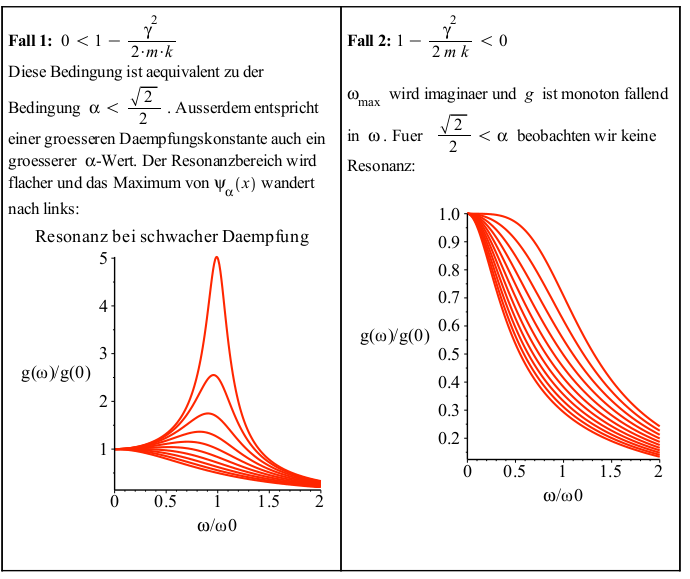
\includegraphics[width=1.0\textwidth]{images/Erzwungen1.png}
\end{minipage}
\begin{minipage}[h]{0.5\textwidth}
	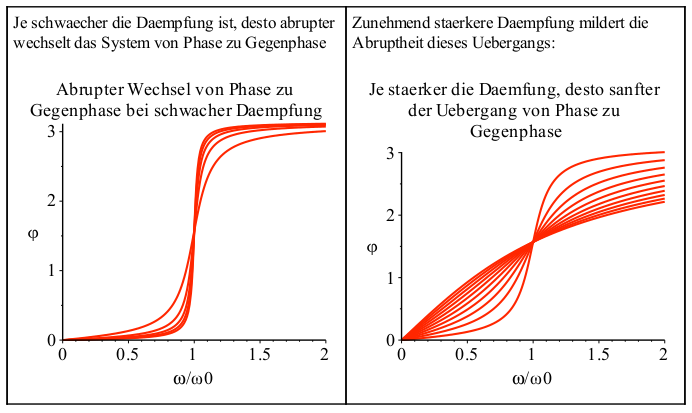
\includegraphics[width=1.0\textwidth]{images/Erzwungen2.png}
\end{minipage}

\subsection{Steife Systeme}
$	\lvert\frac{\lambda_1}{\lambda_2}\rvert \gg 1 \rightarrow \mathrm{impliziter Euler}$

